\documentclass[letter, 10pt]{article}
\usepackage{fullpage}
\usepackage[margin=0.5in]{geometry}
\usepackage{graphicx}
\usepackage{caption}
\usepackage{subcaption}
\usepackage[table]{xcolor}
\usepackage{amsmath}
\usepackage{listings}
\usepackage{float}
\usepackage{array,multirow}
\usepackage{tikz}
\usepackage{cancel}
\usepackage{listings}
\setcounter{MaxMatrixCols}{20}
\usetikzlibrary{arrows}
\pagenumbering{gobble}
\usepackage{diagbox}
\begin{document}
\noindent
\large \textbf{Rahul Ghosh} \hfill \textbf{Assignment\#5}\\
\normalsize Student ID: 5476965 \hfill CSci 5512\\

\section*{Question 1}
\begin{lstlisting}[language=Python]
"""
Created on Sun Apr 28 12:19:33 2019
@author: ghosh128
"""
import pandas as pd
import numpy as np
from scipy.stats import entropy as sc_entropy

df=pd.read_csv('inTree.csv', sep=',')
attribute_names = df.columns[1:-1].values
array = df.values[:, 1:]
array = array.astype(int)
X = array[:, :-1]
Y = array[:, -1]
tree = [None]*(np.power(2,X.shape[1]+1))

def entropy(Y):
    value,counts = np.unique(Y, return_counts=True)
    ent = sc_entropy(counts, base=2)
    return ent

def makeTree(X, Y, index):
    if len(np.unique(Y))==1:
        tree[index] = str(np.unique(Y)[0])
        return
    else:
        before_ent = entropy(Y)
        gain = []
        for attribute in range(X.shape[1]):
            left = Y[X[:,attribute]==1]
            left_ent = entropy(left)
            right = Y[X[:,attribute]==0]
            right_ent = entropy(right)
            attribute_ent = len(left)/(len(left)+len(right))*left_ent +
                            len(right)/(len(left)+len(right))*right_ent
            gain.append(before_ent-attribute_ent)
        attribute = np.argmax(gain)
        tree[index] = attribute_names[attribute]
        makeTree(X[X[:,attribute]==1, :], Y[X[:,attribute]==1], 2*index)
        makeTree(X[X[:,attribute]==0, :], Y[X[:,attribute]==0], 2*index + 1)

makeTree(X, Y, 1)
index = np.power(2,len(attribute_names)+1)-1
while index>=0:
    if tree[index] is not None:
        break
    index -= 1
index = np.power(2, int(np.log2(index))+1)
tree = np.array(tree[1:index])
tree[list(np.where(np.array(tree) == None)[0])] = " "
tree = list(tree)

print("_".join(tree))
\end{lstlisting}
\newpage

\section*{Question 2}
\begin{tabular}{ |c|c|c| } 
    \hline
    \backslashbox{A}{O} & F & T \\
    \hline
    F & 7 & 4 \\
    \hline
    T & 2 & 7 \\ 
    \hline
\end{tabular}\qquad
\begin{tabular}{ |c|c|c| } 
    \hline
    \backslashbox{B}{O} & F & T \\
    \hline
    F & 5 & 3 \\
    \hline
    T & 4 & 8 \\ 
    \hline
\end{tabular}\qquad
\begin{tabular}{ |c|c|c| } 
    \hline
    \backslashbox{C}{O} & F & T \\
    \hline
    F & 4 & 8 \\
    \hline
    T & 5 & 3 \\ 
    \hline
\end{tabular}\qquad
\begin{tabular}{ |c|c|c| } 
    \hline
    \backslashbox{D}{O} & F & T \\
    \hline
    F & 6 & 3 \\
    \hline
    T & 3 & 8 \\ 
    \hline
\end{tabular}\qquad
\begin{tabular}{ |c|c|c| } 
    \hline
    \backslashbox{E}{O} & F & T \\
    \hline
    F & 7 & 3 \\
    \hline
    T & 2 & 8 \\ 
    \hline
\end{tabular}


Accuracy of combinations of 3 attributes by doing majority voting:
\begin{itemize}
    \item[-] {A,B,C} : 15/20
    \item[-] {A,B,D} : 16/20
    \item[-] {A,B,E} : 16/20
    \item[-] {A,C,D} : 20/20
    \item[-] {A,C,E} : 16/20
    \item[-] {A,D,E} : 17/20
    \item[-] {B,C,D} : 15/20
    \item[-] {B,C,E} : 13/20
    \item[-] {B,D,E} : 17/20
    \item[-] {C,D,E} : 17/20
\end{itemize}
The combination of A ,C \& D gives the highest accuracy.
\newpage

\section*{Question 3}
\begin{itemize}
    \item For Node $(1T, 8F) \rightarrow (1T,1F)(0T,7F)$
    \begin{equation*}
        x = \frac{(1-\frac{2}{9})^2}{\frac{2}{9}} + \frac{(1-\frac{16}{9})^2}{\frac{16}{9}} + \frac{(0-\frac{7}{9})^2}{\frac{7}{9}} +\frac{(7-\frac{56}{9})^2}{\frac{56}{9}} = 3.9375 \qquad \chi^2_1(x) = \chi^2_1(3.9375) = 0.95
    \end{equation*}

    \item For Node $(5T, 3F) \rightarrow (3T,0F)(2T,1F)(0T,2F)$
    \begin{equation*}
        x = \frac{(3-\frac{15}{8})^2}{\frac{15}{8}} + \frac{(0-\frac{9}{8})^2}{\frac{9}{8}} + \frac{(2-\frac{15}{8})^2}{\frac{15}{8}} +\frac{(1-\frac{9}{8})^2}{\frac{9}{8}} +\frac{(0-\frac{5}{4})^2}{\frac{5}{4}} +\frac{(2-\frac{3}{4})^2}{\frac{3}{4}} = 5.155 \qquad \chi^2_1(x) = \chi^2_1(5.155) = 0.98
    \end{equation*}

    \item For Node $(1T, 1F) \rightarrow (1T,0F)(0T,1F)$
    \begin{equation*}
        x = \frac{(1-\frac{1}{2})^2}{\frac{1}{2}} + \frac{(0-\frac{1}{2})^2}{\frac{1}{2}} + \frac{(0-\frac{1}{2})^2}{\frac{1}{2}} +\frac{(1-\frac{1}{2})^2}{\frac{1}{2}} = 2 \qquad \chi^2_1(x) = \chi^2_1(2) = 0.84
    \end{equation*}

    \item For Node $(2T, 1F) \rightarrow (2T,0F)(0T,1F)$
    \begin{equation*}
        x = \frac{(2-\frac{4}{3})^2}{\frac{4}{3}} + \frac{(0-\frac{2}{3})^2}{\frac{2}{3}} + \frac{(0-\frac{2}{3})^2}{\frac{2}{3}} +\frac{(1-\frac{1}{3})^2}{\frac{1}{3}} = 3 \qquad \chi^2_1(x) = \chi^2_1(3) = 0.92
    \end{equation*}
\end{itemize}
Therefore the split at nodes (1T,1F) \& (2T,1F) can be removed.

\begin{figure}[H]
    \centering
    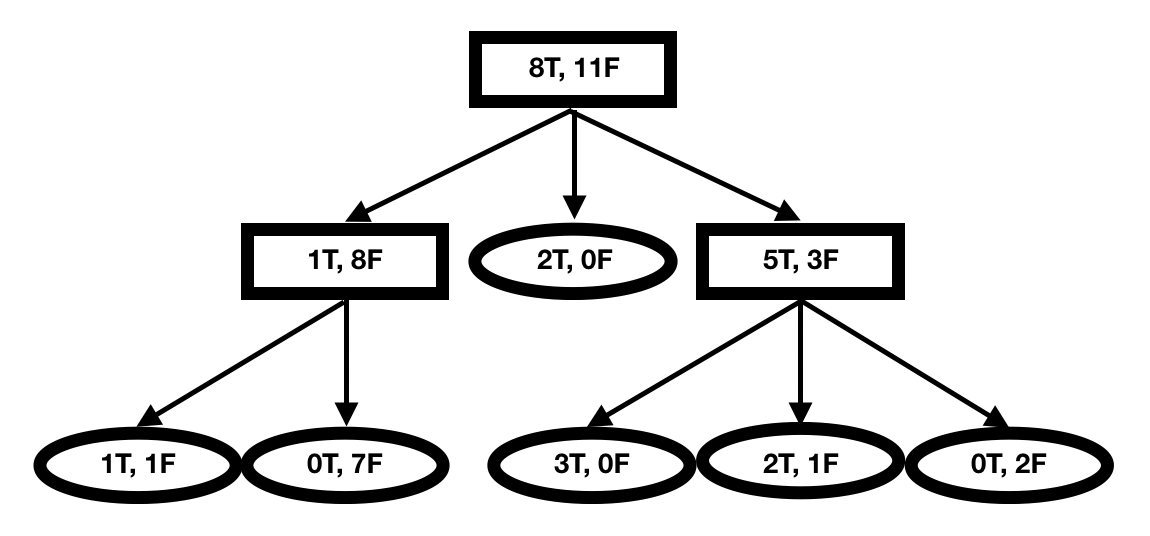
\includegraphics[width=\linewidth]{HW5/PRUNED_TREE.png}
    \caption{Pruned Tree}
    \label{fig:Pruned Tree}
\end{figure}
\newpage

\section*{Question 4}
\begin{align*}
    N1 &= \dfrac{1}{1 + e^{-(w_1\times in_1 + w_2\times in_2)}} = \dfrac{1}{1 + e^{-(0.5\times 0.6 + 0.3\times 0.5)}} = \dfrac{1}{1 + e^{-0.45}} = 0.61\\
    N2 &= \dfrac{1}{1 + e^{-(w_3\times in_2 + w_4\times in_3)}} = \dfrac{1}{1 + e^{-(0.4\times 0.5 + 0.6\times 0.3)}} = \dfrac{1}{1 + e^{-0.38}} = 0.59\\
    N3 &= \dfrac{1}{1 + e^{-(w_5\times N1)}} = \dfrac{1}{1 + e^{-(1\times 0.61)}} = \dfrac{1}{1 + e^{-0.61}} = 0.65\\
    N4 &= \dfrac{1}{1 + e^{-(w_6\times N1 + w_7\times N2)}} = \dfrac{1}{1 + e^{-(0.7\times 0.61 - 0.3\times 0.59)}} = \dfrac{1}{1 + e^{-0.25}} = 0.56\\
    N5 &= \dfrac{1}{1 + e^{-(w_8\times N3 + w_9\times N4)}} = \dfrac{1}{1 + e^{-(-0.5\times 0.65 + 0.9\times 0.56)}} = \dfrac{1}{1 + e^{-0.18}} = 0.55\\
\end{align*}
\begin{equation*}
    f(x) = \frac{1}{1+e^{-x}} \implies \frac{\partial f(x)}{\partial x} = f\times(1-f)
\end{equation*}
\begin{align*}
    out =& 1\\
    Error =& \frac{(out - N5)^2}{2}\\
    \frac{\partial Error}{\partial w_9} =& \frac{\partial Error}{\partial N5}\frac{\partial N5}{\partial (w_8\times N3 + w_9\times N4)}\frac{\partial (w_8\times N3 + w_9\times N_4)}{\partial w_9} = -(out-N5)(N5(1-N5))(N4)\\=& -(1-0.55)(0.55(1-0.55))(0.56) = -0.06237\\
    w_9 =& w_9 - \alpha \frac{\partial Error}{\partial w_9} = 0.9 + 0.5\times0.06237 = 0.931185
\end{align*}

\section*{Question 5}
\begin{align*}
    out =& 1\\
    Error =& \frac{(out - N5)^2}{2}\\
    \frac{\partial Error}{\partial w_1} =& \frac{\partial Error}{\partial N5}\frac{\partial N5}{\partial (w_8\times N3 + w_9\times N4)}
    \begin{bmatrix} 
        \frac{\partial (w_8\times N3 + w_9\times N4)}{\partial N3} & \frac{\partial (w_8\times N3 + w_9\times N4)}{\partial N4} 
    \end{bmatrix}
    \begin{bmatrix} 
        \frac{\partial N3}{\partial (w_5\times N1)} & \frac{\partial N4}{\partial (w_5\times N1)}\\
        \frac{\partial N3}{\partial (w_6\times N1 + w_7\times N2)} & \frac{\partial N4}{\partial (w_6\times N1 + w_7\times N2)}
    \end{bmatrix}\\
    &\begin{bmatrix} 
        \frac{\partial (w_5\times N1)}{\partial N1}\\
        \frac{\partial (w_6\times N1 + w_7\times N2)}{\partial N1} 
    \end{bmatrix}
    \frac{\partial N1}{\partial (w_1\times in_1 + w_2\times in_2)}\frac{\partial (w_1\times in_1 + w_2\times in_2)}{\partial w_1}\\
    =& -(out - N5)(N5(1-N5))
    \begin{bmatrix} 
        w_8 & w_9
    \end{bmatrix}
    \begin{bmatrix} 
        N3(1-N3) & 0\\
        0 & N4(1-N4)
    \end{bmatrix}
    \begin{bmatrix} 
        w_5\\
        w_6
    \end{bmatrix}
    (N1(1-N1))(in_1)\\
    =& -(1-0.55)(0.55(1-0.55))
    \begin{bmatrix} 
        -0.5 & 0.9
    \end{bmatrix}
    \begin{bmatrix} 
        0.65(1-0.65) & 0\\
        0 & 0.56(1-0.56)
    \end{bmatrix}
    \begin{bmatrix} 
        1\\
        0.7
    \end{bmatrix}
    (0.61(1-0.61))(0.6)\\
    =& -(1-0.55)(0.55(1-0.55))(-0.5\times0.65(1-0.65)\times(1) + 0.9\times0.56(1-0.56)\times0.7)(0.61(1-0.61))(0.6)\\
    =& -0.00066\\
    w_1 =& w_1 - \alpha \frac{\partial Error}{\partial w_1} = 0.5 + 0.5\times0.00066 = 0.5033
\end{align*}
\newpage

\section*{Question 6}
\begin{equation*}
    f(a,b,c,d) = 2a^2c^4 - ab + e^{sin(d)+d} + 2b^2d^2 - 3c^3d
\end{equation*}
\begin{align*}
    \frac{\partial f}{\partial a} &= 4ac^4 - b\\
    \frac{\partial f}{\partial b} &= - a + 4bd^2\\
    \frac{\partial f}{\partial c} &= 8a^2c^3 - 9c^2d\\
    \frac{\partial f}{\partial d} &= e^{sin(d)+d}(cos(d) + 1) + 4b^2d - 3c^3\\
\end{align*}
$\alpha = 0.01$
\begin{align*}
    & a = a - \alpha* \frac{\partial f}{\partial a} = a - 0.01\times(4ac^4 - b)\\
    & b = b - \alpha* \frac{\partial f}{\partial b} = b - 0.01\times(4bd^2 - a)\\
    & c = c - \alpha* \frac{\partial f}{\partial c} = c - 0.01\times(8a^2c^3 - 9c^2d)\\
    & d = d - \alpha* \frac{\partial f}{\partial d} = d - 0.01\times(e^{sin(d)+d}(cos(d) + 1) + 4b^2d - 3c^3)\\
\end{align*}
With number of iterations equal to 100000, the final values that we get is a=0, b=0, c=0 and d=3.141. The values of a with respect to the iteration are shown in figures below.
\newpage
\end{document}